\documentclass{standalone}
\usepackage{tikz}
\usetikzlibrary{3d,shapes.geometric,calc}


\begin{document}
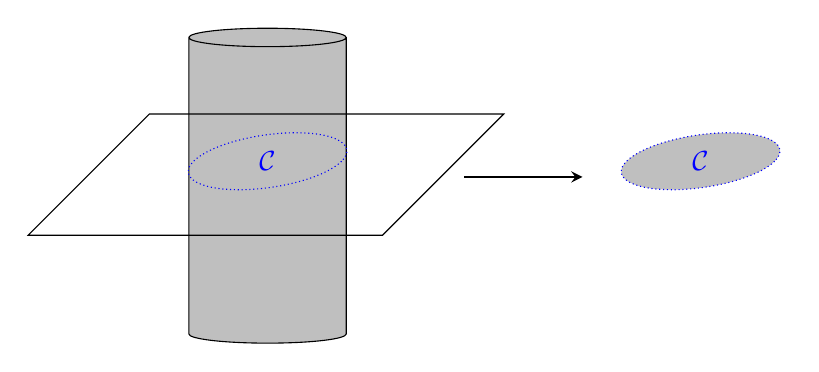
\begin{tikzpicture}[scale=2]
  \node [canvas is xy plane at z=0,
	cylinder,
	fill=gray!50!white, 
	rotate=90,
	draw,
	minimum height=4cm,
	minimum width=2cm] (c) at (0,0) {};
  \draw[canvas is xz plane at y=0.5] (-.75,0) rectangle (1.5,2);
  \draw[blue,densely dotted, canvas is xz plane at y=0.2] (0,0) node {$\mathcal{C}$} circle (0.47);
  
  \draw [thick,->,>=stealth] (1.25,0.1) -- (2,0.1);
  \draw[blue,fill=gray!50!white,densely dotted, canvas is xz plane at y=0.2] (2.75,0) node {$\mathcal{C}$} circle (0.47);
\end{tikzpicture}


\end{document}